\section{Beräkna Antalet Nollställen}
Detta är en väldigt vanlig uppgift på tentan, vad jag kan se så har den varit med på alla tentor som ligger ute. Uppgiften brukar vara formulerad ungefär såhär 
Här är annan text. 
\begin{tcolorbox}
Bestäm antalet nollställen som polynomet 
\begin{align*}
	p(z) = ...
\end{align*}
har i området ... (oftast ett halvplan)
\end{tcolorbox} 


Ett spciallfall som kan vara värt att undersöka är ifall $p(z)$ har något nollställe som är rent reelt eller rent imaginärt och om detta ligger på $L_R$ eller $I_R$. Om så är fallet så ingår inte denna i området och man behöver faktorisera bort detta nollställe innan man börjar sina beräkningar. Man kommer då att få ett polynom $q(z)$ som är minst en grad mindre än $p(z)$ vilket är det polynom man ska göra resterande beräkningar på. 

\subsection{Antal Nollställen I Halvplan/Kvadrant }
Det första steget är att rita upp situationen. Man gör detta genomom att beskriva området som en tårtbit.
\begin{center}
\begin{tikzpicture}
	\draw[->] (0,0) -- (1.5,0);
	\draw[->] (0,0) -- (0,1.5);
	\draw[->] (0,0) -- (-1.5,0);
	\draw[->] (0,0) -- (0,-1.5);
	\draw[very thick] (0,1) arc (90:0:1);
\end{tikzpicture}
\qquad
\begin{tikzpicture}
	\draw[->] (0,0) -- (1.5,0);
	\draw[->] (0,0) -- (0,1.5);
	\draw[->] (0,0) -- (-1.5,0);
	\draw[->] (0,0) -- (0,-1.5);
	\draw[very thick] (-1,0) arc (180:0:1);
\end{tikzpicture}
\qquad
\begin{tikzpicture}
	\draw[->] (0,0) -- (1.5,0);
	\draw[->] (0,0) -- (0,1.5);
	\draw[->] (0,0) -- (-1.5,0);
	\draw[->] (0,0) -- (0,-1.5);
	\draw[very thick] (-1,0) arc (-180:0:1);
\end{tikzpicture}
\end{center}
Där man låter radien, $R \rightarrow \infty$. På detta sätt skapas en tårtbit som täcker in hela området. Det finns konventioner i kursen för hur dessa linjer och bågar ska namnges. Bågelementet kallas $C_R$, sträckan på den realla axeln kallas $L_R$ och sträckan på den imaginära axeln kallas $I_R$. Som man kan se i bilden så är det möjligt att ett område bara har en av dessa sträckor, om vinkeln på bågelementet är $\pi$.

Nästa steg är att nogrant tänka ut riktningen på dessa sträckor och bågar. Dessa riktningar bestämmer tecknet då man ska räkna ut det totala tillskottet som det inneslutna området $\Gamma_R$ utgör. För de tre bilderna ovan får vi
\begin{align*}
	\Gamma_R =& C_R + L_R + I_R \\
	\Gamma_R =& C_R + L_R \\
	\Gamma_R =& C_R - L_R
\end{align*}
Håller man tungan rätt i mun kan man göra detta på flera sätt. Jag föredrar att alltid låta $L_R$ och $I_R$ peka åt höger respektive uppåt, medans $C_R$ alltid har positiv riktning. \\

\subsubsection*{Bågelementets Bidrag}
Nästa steg är att beräkna bidraget som bågelementet utgör. Detta uttrycks
\begin{align*}
	\Delta_{C_R} \arg p(z)
\end{align*}
Vad man ofta uttnyttjar är att operationen $\arg$ har egenskapen 
\begin{align*}
	\arg \left( p(z) g(z) \right) = \arg p(z) + \arg g(z)
\end{align*}
Vad man gör är att bryta ut den största exponeneten. Om man använder ett godtyckligt polynom som exempel får man någos i stil med
\begin{align*}
	\Delta_{C_R} \arg \left( z^3 + 4z^2 + z + 3 \right) = \Delta_{C_R} \arg z^3 + \Delta_{C_R}\arg \left( 1+4/z+1/z^2 + 3/z^3 \right)
\end{align*}

När $R \rightarrow \infty$ så kommer den högra termen att gå mot $\arg 1 = 0$. Så i detta exempel så försvann denna termen helt, vilket den gjort i alla exempel jag undersökt. Nästa steg blir att beräkna termen som är kvar, för detta kan vi använda en annan trevlig egenskap hos $\arg$-operationen.
\begin{align*}
	\Delta_{C_R} \arg z^n = n \Delta_{C_R} \arg z 	
\end{align*}
Vi vet vad n är och $\Delta_{C_R} \arg z$ är helt enkelt argumentet för bågelementet. Nu vet vi bågelemtets tillskot. \\

\subsubsection*{Sträckornas Bidrag}
Nästa steg är att beräkna tillskottet för sträckan eller sträckorna som skapar det inslutna området tillsammans med bågelementet. Om vi går tillbaks till bilden i början avsnittet så finns det här lite olika fall. I den första bilden så behöver två sträckor undersökas. Dessa undersöks separat genom att ersätta $z$ med $x$ respektive $iy$. Man får då två polynom
\begin{align*}
	p(x) = ... = u(x) + iv(x) \\
	p(iy) = ... = u(y) + iv(y)
\end{align*}
\textbf{Fall 1: Bild 1} \\
Detta kanske är det lurigaste fallet, i alla fall om några av konstanterna i polynomet är koplexa. Är de inte det så är i alla fall realdelen tämligen lättberäknad. Vad man behöver göra är att beräkna $\Delta_{L_R + I_R} \arg p(z)$. Som tur är så börjar den ena där den andra slutar, så man kan räkna dem i "serie". I vårat exempel så börjar man med att göra ett teckenstudie för $u+iv$ då $x: R \rightarrow 0$ och för $y:0 \rightarrow R$. Det är då som att man får ett teckenstudie som slutar i 0 och ett som börjar där, på detta vis kan man rita ut kurvan i uv-planet för. Från denna kurva ska man sedan kunna avläsa argumentet för $\Delta_{L_R + I_R}$. \\

\textbf{Fall2: Bild 2 och 3} \\
I dessa fall behöver man bara ansätta ett polynom, $p(x)$ eller $p(iy)$ beroende på om sträckan är horizontel eller vertikal. Sedan gör man om polynomet på formen $u+iy$ och gör teckenstudie mellan $x/y: -R \rightarrow R$. Fråen detta ska man kunna rita kurvan och avläsa argumentet för sträckan. \\

\textbf{Speciallfall, vinkel inte multipel av $\pi/2$} \\
I dessa fall får man göra en parimatisering med en variabel $t$ och ansätta $t+it$ i polynomet, om vinkeln skulle vara $\pi/4$. \\

\subsection*{Sätta Ihop Allt}
Nu har vi kommit till det slutgiltiga steget, att addera alltihop och se reslultatet. Detta brukar uttryckas
\begin{align*}
	\lim_{z \rightarrow R} \frac{1}{2 \pi} \Delta_{C_R + L_R + I_R} \arg p(z)
\end{align*}
Vad detta innebär är att man adderar alla argument man räknat ut innan, eller subtraherar om elementet är negativt, och delar alltihop med $2 \pi$, svaret är antalet nollställen minus antalet poler. \\


\subsection{Antalet Nollställen I En Cirkelskiva}
Detta är också en vanlig uppgift vad gäller beräkning av antalet nollställen i ett område. Det är vanligt att detta är en deluppgift och man använder samma polynom i båda uppgifterna. Det kommer antas att man lånar många koncept från tidigare avsnitt, så allt förklaras inte här. Uppgifter uttrycks ofta något i stil med

\begin{tcolorbox}

Bestäm antalet nollställen som polynomet 
\begin{align*}
	p(z) = ...
\end{align*}

	har på (enhet) skivan $|z| < r$

\end{tcolorbox}
Området får då utseendet. 
\begin{center}
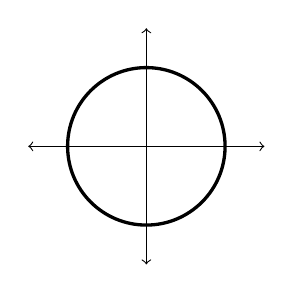
\begin{tikzpicture}
	\draw[->] (0,0) -- (1.5,0);
	\draw[->] (0,0) -- (0,1.5);
	\draw[->] (0,0) -- (-1.5,0);
	\draw[->] (0,0) -- (0,-1.5);
	\draw[very thick] (1,0) arc (360:0:1);
\end{tikzpicture}
\end{center}
Man kan redan börja misstänka att denna kalkyl har med polära koordinater att göra, och det har det. När man löser denna typen av uppgift så ersätter man $z$ med $e^{i \theta}$. Man sätter in detta i polynomet och uttrycker det hela på $u + iv$ -form. Detta steg kräver att man gör om alla termer till cos och sinus, för att kunna dela upp dessa delar. \\

När man delat upp alla delar så görs ett teckenstudie mellan $-\pi$ och $\pi$, där man är noggran med att undersöka alla nollställen på vägen för både u och v. Därefter används argumentprincipen, som i tidigare avsnitt.  
